\section{Power System}
In order for the segway to know its location in the maze and map it accordingly, it will need some reference points in the demo arena for it to recognize. This will be in the form of three LED beacons that may be placed anywhere around the arena.

\subsection{Power Supply}
The power supply of the whole DC grid is provided by solar energy. Throughout the project, PV panels are used as the power supply of the DC grid. However, since the actual run of the device will be in an undesirable environment for PV panels, a power supply unit will be used to emulate the performance of the PV panels.

To start off, the performance of the PV panels is tested. IV characteristics are plotted for PV panels in different configurations. The ratings of individual PV panels are given as 5V and 230mA.

The data in the figures are taken in a sunny day in a bright environment. The result is as expected. The IV characteristic exhibits a flat line at lower voltage and a steep drop and higher voltage. This also results in a PV graph that has a shape as expected. The power increases linearly at lower voltage and drops drastically at higher voltage. This leads to the maximum power point of the PV panels. The maximum output power of the PV panels is given at around 4.5V to 5V.

\begin{figure}
    \centering
    \begin{subfigure}[b]{.45\linewidth}
        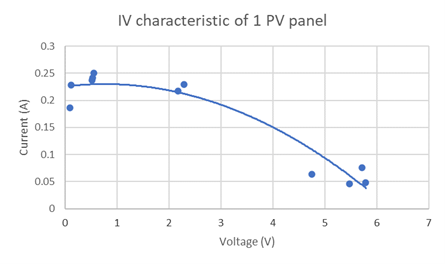
\includegraphics[width=\linewidth]{images/iv-1.png}
    \end{subfigure}
    \begin{subfigure}[b]{.45\linewidth}
        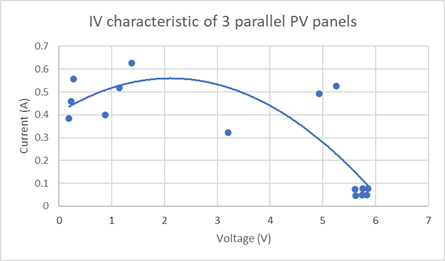
\includegraphics[width=\linewidth]{images/iv-3.png}
    \end{subfigure}
    \begin{subfigure}[b]{.45\linewidth}
        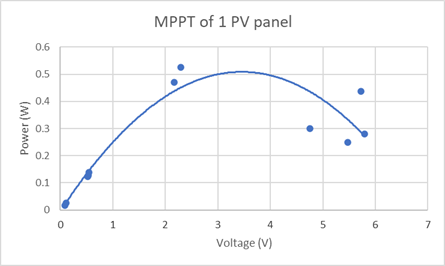
\includegraphics[width=\linewidth]{images/mppt-1.png}
    \end{subfigure}
    \begin{subfigure}[b]{.45\linewidth}
        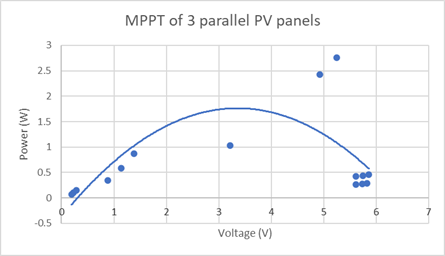
\includegraphics[width=\linewidth]{images/mppt-3.png}
    \end{subfigure}
    \caption{MPPT and IV characteristics of PV panels in different configurations}
    \label{fig:mppt}
\end{figure}

From figure \ref{fig:mppt} above, showing the IV characteristics of a single PV panel, has the expected trend for a maximum current of 0.24mA and drops at around 4V. When compared to figure which shows the IV characteristics of three PV panels in parallel, the shape of both graphs is similar. However, the parallel configuration produces a much higher output current, which leads to a higher output power. Higher output current is desired since quite a lot of current is needed to drive three LEDs in parallel. Series configuration has also been tested at the same day. However, it is not ideal to use it although it gives a much higher voltage. Its output current is very unreliable and has a large fluctuation of output voltage. If anyone of the PV panels is half covered, the output voltage and current drops significantly, which is undesirable as a power supply.

The PV panels are also connected to a boost switch mode power supply (SMPS) for further testing to simulate the real demonstration. Three parallel PV panels are connected to a boost SMPS and a 75\(\Omega\) load, or a 10\(\Omega\) for lower voltages, to create an IV characteristic for the PV panels with a boost SMPS connected and a load. The result are shown in figure \ref{fig:mppt-load}.

\begin{figure}
    \centering
    \begin{subfigure}[b]{.45\linewidth}
        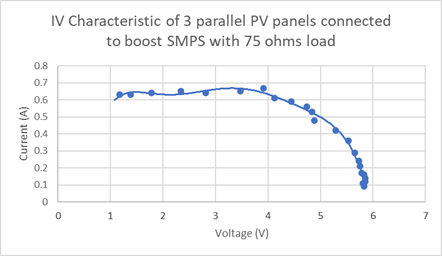
\includegraphics[width=\linewidth]{images/iv-3-load.png}
    \end{subfigure}
    \begin{subfigure}[b]{.45\linewidth}
        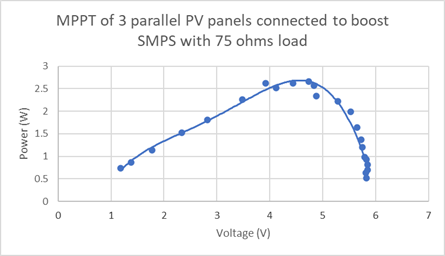
\includegraphics[width=\linewidth]{images/mppt-3-load.png}
    \end{subfigure}
    \caption{}
    \label{fig:mppt-load}
\end{figure}

The results are as expected. The IV characteristic shows a plateau at lower voltages with around 0.65 mA and has a significant drop at larger than 5V. This results in an expected graph of power, which shows that the maximum output power would be around 4V to 5V.

\subsection{Maximum Power Point Tracking}

\begin{figure}
    \footnotesize
    \begin{minted}{python}
power1 = vb * iL;
power_diff = power1 - power0;
power0 = power1;
vb_diff = vb - vb_old;
vb_old = vb;
if (power_diff > 0){
    if(vb_diff > 0){
        open_loop=open_loop-0.001;
    }
    else{
        open_loop=open_loop+0.001;
    }
}
else{
    if(vb_diff > 0){
        open_loop=open_loop+0.001;
    }
    else{
        open_loop=open_loop-0.001;
    }
}
    \end{minted}
    \caption{}
    \label{code:pert_observe}
\end{figure}

Maximum power point tracking (MPPT) is used mainly to maximize the power output from the PV panels by adjusting the operating point. The algorithm continuously monitors the output voltage and current and adjusts the operating point. This ensures the system to harvest the maximum power from the PV panels for most of the conditions. This will negate small oscillations coming from the current supply due to weather conditions such as a cloud blocking the sun. The algorithm is implemented in a perturb and observe method~\cite{ref:mppt}. The code implemented is shown in figure \ref{code:pert_observe}. The code gets the current value and past value of voltage and current and compares them. When the power and voltage are both larger, it means that it has not reached it’s maximum power, and duty cycle is further increased. In the code, the duty cycle is decreased. This is correct since the PMOS is the boost SMPS reverses the operation. The algorithm ensures that the power in the DC grid will be as high as possible at any given time, given a steady brightness of the LED beacons as much as possible.


\subsection{LED}

The main component of the energy system are the three LED beacons, which will be essential to help the robot to navigate through the maze. There are three different colours of LED, red, blue and yellow. The exact ratings of the LEDs are not given except for 1W. Preliminary testing is needed to find out the diode drop, maximum voltage and current of each colour of the LEDs. Initially the LED beacons are run from a power supply unit at a voltage of 2V and the current limit to approximately 50mA. After that, the voltage limit is brought up until the voltage will rise to a fixed value. That value is the voltage drop of the diode. After that, the current is brought up such that the diode consumes 0.9W. That will be the expected maximum brightness of the LED. The voltage drop at lower current levels are also plotted for reference. The maximum operating point is purposedly tested at 0.9W. This prevents unexpected situations that will break the LEDs. Data is taken from the display of the power supply unit. The experimental results are in figure \ref{tbl:led}.

\begin{figure}
    \centering
    \begin{tabular}{ |c|c|c|c|}
        \hline
                            & Yellow & Blue  & Red   \\
        \hline
        Diode Voltage (V)   & 1.95   & 2.69  & 1.95  \\
        \hline
        Maximum Voltage (V) & 2.32   & 3.09  & 2.41  \\
        \hline
        Maximum Current (A) & 0.427  & 0.311 & 0.376 \\
        \hline
    \end{tabular}
    \caption{}
    \label{tbl:led}
\end{figure}

\begin{figure}
    \centering
    \begin{subfigure}[b]{.3\linewidth}
        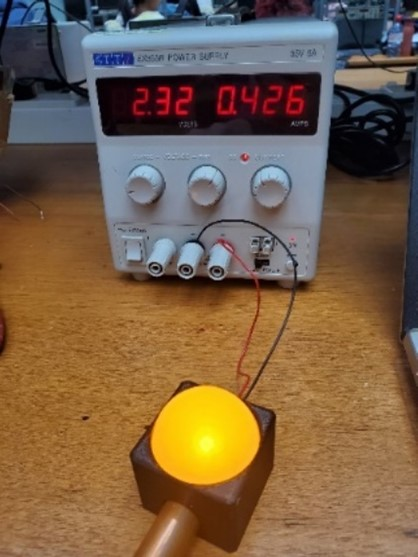
\includegraphics[width=\linewidth]{images/led-yellow.jpg}
    \end{subfigure}
    \begin{subfigure}[b]{.3\linewidth}
        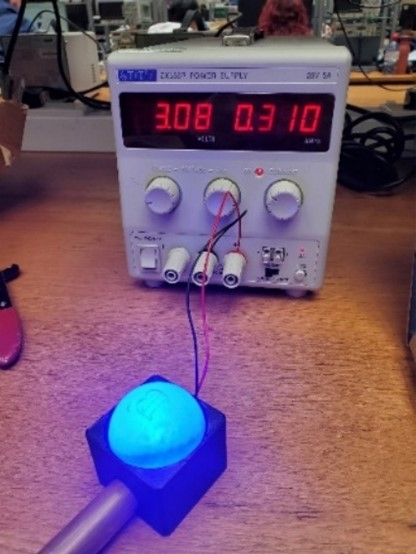
\includegraphics[width=\linewidth]{images/led-blue.jpg}
    \end{subfigure}
    \begin{subfigure}[b]{.3\linewidth}
        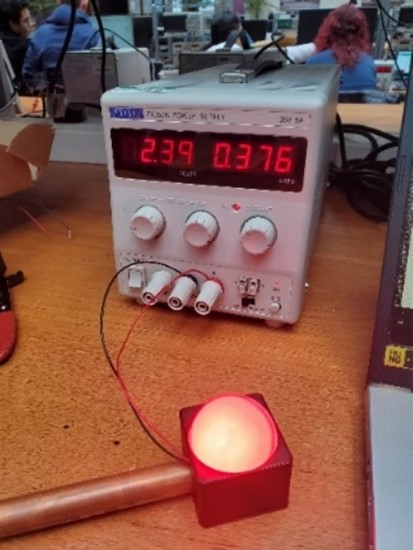
\includegraphics[width=\linewidth]{images/led-red.jpg}
    \end{subfigure}
    \caption{LED Beacons}
\end{figure}

After the initial testing of the LEDs, each of them is connected to a separate LED driver, which is a buck SMPS. It controls how much current can flow through into the LED and prevents it from breaking. For better and stable control of the output from the LED driver, closed-loop buck SMPS is chosen for the LED driver. The advantage of a closed-loop controller is that the output voltage is regulated at a desired value by our command and it does not vary with output current when compared to open-loop buck SMPS.

Proportional-integral-derivative (PID) controller is used in the design. In the implementation of the closed-loop buck SMPS, a PID loop in created within a PID control loop. The inner loop controls the SMPS output current, a reference current is provided by the current sensing resistor at the output side of the LED driver. The current reference is generated by the outer voltage control loop. It uses the output voltage to calculate a voltage error and then demands a current from the inner loop. This results in a good voltage regulation and a high efficiency across a range of output current. Figure \ref{code:pidv} is an excerpt from the controller code of the PID function for controlling the voltage.

\begin{figure}
    \footnotesize

    \begin{minted}{python}
    def pidv(pid_input):
        global e0v, e1v, e2v, u0v, u1v, delta_uv
        e_integration = e0v
        if u1v >= uv_max or u1v <= uv_min:
            e_integration = 0

        delta_uv =  (kpv * (e0v - e1v) + kiv * Ts * 
                    e_integration + kdv / Ts * (e0v - 2 * e1v + e2v)
                    )  
        u0v = u1v + delta_uv

        saturation(u0v, uv_max, uv_min)

        u1v = u0v
        e2v = e1v
        e1v = e0v

        return u0v
    \end{minted}
    \caption{PID control loop for voltage control}
    \label{code:pidv}
\end{figure}

\begin{figure}
    \footnotesize
    \begin{minted}{python}
    def saturation(sat_input, uplim, lowlim):
        if sat_input > uplim:
            sat_input = uplim
        elif sat_input < lowlim:
            sat_input = lowlim

        return sat_input
    \end{minted}
    \caption{Saturation function}
    \label{code:saturation}
\end{figure}

A saturation function is also introduced in the code to prevent overshoot. This is used mainly to limit the duty cycle so that it does not fall below 0 or go above 1. It is also used as a safety net to prevent too much current going through the output into the LED.

The result of the controller is that the input of LED driver could work up to 15V without the LED breaking on the output side. This is sufficiently enough since the LEDs would not be wanted to work on the edge of breaking and the voltage limit on the LED drivers is 18V. Moreover, the output of the boost SMPS does not allow such high voltage. Therefore, the design of the LED drivers is safe enough to not break.

\subsection{Initial Design}

\begin{wrapfigure}{r}{0.4\textwidth}
    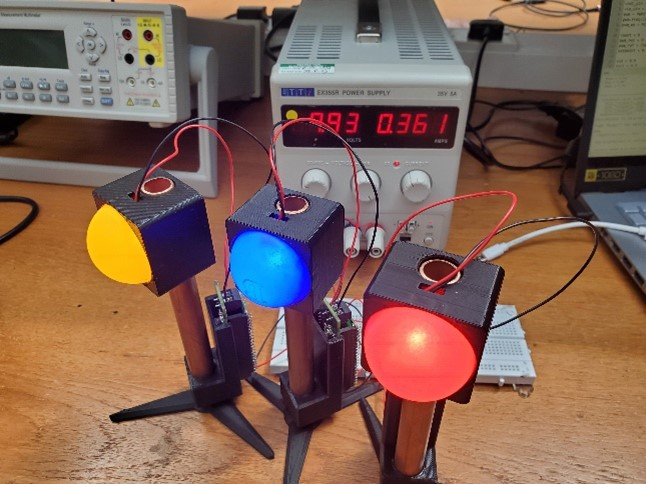
\includegraphics[width=0.38\textwidth]{images/all-leds.jpg}
\end{wrapfigure}

After testing out each of the LED drivers with LED lights, three of them are put together in parallel connect to the power supply. The test is operated at a voltage of 10V. All 3 of the LED beacons are successfully lit up. The next step is to the with an emulated PV panel with a power supply. Previously, the boost SMPS with PV panels and each of the LED beacons are tested separately and each of them are working as intended. When combined into a circuit, it is expected to light the LED beacons up. To emulate PV panels, the current limit is set to 0.7A and the voltage is changed from 4V to 5V.

The circuit is working as intended. All three LED beacons light up. When the voltage is at 5V, the beacons are lit up as expected as is operating with around 0.7W to 0.8W. This ensures that the LEDs do not get overpowered and breaks. When the voltage is at 4V, the beacons are still lit up but is very dim. Although the camera could still pick up and differentiate the three colours in the state, it is not ideal since the lights are on the verge of turning off and it is very prone to unexpected circumstances.

To solve the problem, a supercapacitor is introduced in parallel to the three LED beacons. The theory of the part of the supercapacitor is that when the voltage in the DC electricity grid changes, it is able to react and counteract to the change in voltage. When the voltage in the electricity grid is higher than a pre-set reference, the supercapacitor will charge up from the excess voltage in the DC grid. When the voltage in the electricity grid is lower than the pre-set reference, the supercapacitor will discharge into the electricity grid to compensate for the low voltage. This ideally keeps the DC electricity grid at a relatively constant voltage, which eliminates the problem of the brightness of the LED beacons varying with the voltage of the DC grid.

In theory, a bi-directional SMPS could be implemented for this supercapacitor. The code for the controller can be designed so that it can switch between buck and boost depending on the voltage at the port connected to the DC electricity grid. When the voltage is higher than the reference point, the SMPS will be in buck mode. The port connecting the DC grid will be the input and step down the voltage to charge up the supercapacitor. When the voltage is lower than the reference point, the SMPS will be in boost mode. The supercapacitor will discharge and the voltage will be boosted into the DC electricity grid. For example, if the power supply is working in the range of 0V to 5V, and the DC electricity grid is around 0V to 15V, the reference could be around 7.5V. This makes half the time charging the capacitor and half the time discharging the capacitor, achieving a more stable DC electricity grid for the LED beacons. This is based on the assumption that there will be half the time more than the average and half the time less than the average.

In reality, the bi-directional SMPS was not provided in time, resulting in the brightness of the LED beacons highly dependent on the supplied voltage. This is not ideal since the LED turns off when the power supply is at 4V. The LED needs to be lit up as long as possible for better navigation for the robot. For testing purposes, the supercapacitor is connected directly to the DC electricity grid to see its effects on the whole circuit. When the switch is turned on, the LED beacons did not light up immediately. Instead, the LED beacons turn on gradually. This is due to the supercapacitor gradually charging up from the supplied voltage. The voltage of the DC electricity grid increases gradually to 9V, in which the LED beacons turn on at around 1 second after switching on and charges up fully at 2 seconds. When the power supply is turned off, the LED dims out gradually.

\subsection{Evaluation}

As mentioned above, the bi-directional SMPS was not provided in time for any testing with the supercapacitor. This results in the supercapacitor directly connected to the DC grid, which mean that it could not be controlled to charge and discharge relative to the DC grid. However, the EE2 lab SMPS can actually be modified to a bi-directional SMPS. The switch on the SMPS for buck and boost can be bypassed through modifications in the controller code. Unfortunately, due to time constrains, it is not able to do so which results in the lack of testing in the supercapacitor.

